\documentclass[hyperref=colorlinks]{beamer}
\mode<presentation>
\usetheme{iclpt}
\setbeamertemplate{navigation symbols}{}
\setbeamertemplate{headline}{
\begin{beamercolorbox}[leftskip=.2cm,rightskip=.2cm,topskip=.2cm,ht=1.1cm,dp=0.1cm,wd=\textwidth]{institute in head/foot}
  
\includegraphics[height=1cm]{icl.pdf}
  \hfill
  
\includegraphics[height=1cm]{../Pics/CMS-Color.pdf}
\end{beamercolorbox}
}
\setbeamertemplate{footline}{
\begin{beamercolorbox}[ht=.55cm,dp=0.4cm,wd=\textwidth,leftskip=.3cm]{author in head/foot}%
  \begin{minipage}[c]{5cm}%
    \usebeamerfont{author in head/foot}
    \insertshortauthor 
    \insertshorttitle
    \end{minipage}\hfill%
  \insertframenumber{} / \pageref{lastframe}
  \hfill
  \begin{minipage}{6cm}
    \hfill
  \end{minipage}
\end{beamercolorbox}%
}

\usepackage{color}
\usepackage{tabularx,colortbl}
\usepackage{graphicx}
\usepackage{pdfpages}
\usepackage{feynmp}
\usepackage{tikz}
\usetikzlibrary{calc, shapes, backgrounds,arrows,positioning}
\DeclareGraphicsRule{*}{mps}{*}{}

\title{\vspace{-0.2cm} VBF Higgs to Invisible}
\subtitle{HIG-14-038, AN-14-243\vspace{-0.7cm}}
\author[]{}%\underline{P. Dunne}} % A.M. Magnan and A. Nikitenko Joao Pela with \\ R. Aggleton, J. Brooke: Bristol \\ C.Asawangtrakuldee, Q.Li: Peking \\ P. Srimanobhas: Chulalongkorn \\ S. Kumar, K. Mazumdar: Mumbai}
\titlegraphic{
  \vspace{-0.7cm}
  %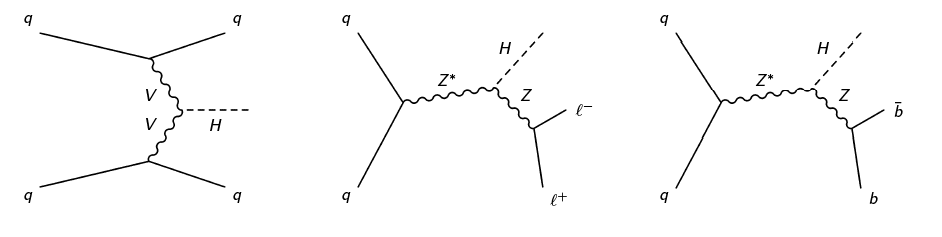
\includegraphics[width=\textwidth]{TalkPics/invcomb021213/feyndiags}
  %% \begin{fmfgraph*}(100,70)
  %%         \fmfleft{i1,i2}
  %%         \fmfright{o1,o2,o3}
  %%         \fmf{fermion}{i1,v1,o1}
  %%         \fmf{fermion}{i2,v2,o3}
  %%         \fmf{phantom,tension=4/5}{v1,v2}
  %%         \fmffreeze
  %%         \fmf{photon,label=$W,,Z$}{v1,v3}
  %%         \fmf{photon,label=$W,,Z$}{v2,v3}
  %%         \fmf{dashes}{v3,o2}
  %%         \fmflabel{$q$}{i1}
  %%         \fmflabel{$q$}{i2}
  %%         \fmflabel{$q$}{o1}
  %%         \fmflabel{$q$}{o3}
  %%         \fmflabel{$H$}{o2}
  %%       \end{fmfgraph*}
}
\date{}
\begin{document}
\begin{fmffile}{higgsexoupdatefeyndiags}
\tikzstyle{every picture}+=[remember picture]

%TITLE PAGE
\section{Title}
\begin{frame}
  \titlepage
  
\end{frame}

\begin{frame}
  \frametitle{Overview}
  \begin{block}{}
    \begin{itemize}
    \item We plan to make ntuples from miniAOD
    \item Working with other ICHiggsTauTau users to update ntuple maker to new recipes
    \item[-] Adinda de Wit, Andrew Gilbert, Rebecca Lane
    \item Will go through progress on objects that have been looked at so far
    \end{itemize}
    \end{block}
\end{frame}

\begin{frame}
  \frametitle{Reminder of framework structure}

  \tikzstyle{format} = [draw, thin, fill=blue!20]
  \tikzstyle{medium} = [ellipse, draw, thin, fill=green!20, minimum height=2.5em]
  \begin{block}{}
    \begin{itemize}
    \item Focus today on miniAOD to ntuples
    \end{itemize}
  \end{block}

  \begin{tikzpicture}[auto,>=latex', thick]
    \path[->] node [format] (AOD) {AOD};
    \path[->] node [format,below of= AOD] (miniAOD) {miniAOD};
    \path[->] node [format,right= 2cm of {$(AOD)!0.5!(miniAOD)$}] (ntuple) {ICHiggsTauTau ntuples}
                  (AOD) edge node {grid} (ntuple);
    \path[->] [ultra thick,red](miniAOD) edge node {grid} (ntuple);
    \path[->] node [format,right= 2cm of ntuple] (lighttree) {Light trees};
    \path[->] (ntuple) edge node {batch job} (lighttree);
    \path[->] node [medium,below= 2cm of {$(ntuple)!0.5!(lighttree)$}] (output) {plots, yields, datacards etc.};
    \path[->] (ntuple) edge node {batch job} (output);
    \path[->] (lighttree) edge node {batch job} (output);
  \end{tikzpicture}
\end{frame}

\begin{frame}
  \frametitle{Electrons}
  \begin{block}{}
    \begin{itemize}
    \item In run 1 we used cut based identification at veto and tight working points
    \item Updated for run 2
    \item[-] Ntuples already contain all required variables
    \item[-] istight() etc. functions will be updated to new cut values
    \item[-] Details \href{https://twiki.cern.ch/twiki/bin/viewauth/CMS/CutBasedElectronIdentificationRun2}{here}
    \end{itemize}
  \end{block}
\end{frame}

\begin{frame}
\frametitle{Muons}
  \begin{block}{}
    \begin{itemize}
    \item In run 1 we used cut based identification at loose and tight working points
    \item[-] These are currently unchanged for run 2
    \item In run 2 there is also a medium working point with better fake rejection than loose but still high efficiency
    \item[-] Ntuples have been updated to contain variables required
    \item Updated for run 2, code has been updated to store all needed variables in ntuples
    \item[-] Details \href{https://twiki.cern.ch/twiki/bin/view/CMS/SWGuideMuonId2015}{here}
    \end{itemize}
  \end{block}
\end{frame}
  
\begin{frame}
  \frametitle{Taus}
  \begin{block}{}
    \begin{itemize}
    \item In run 1 we used same ID as $H\rightarrow\tau\tau$ group
    \item Baseline ID to be used by $H\rightarrow\tau\tau$ in run 2 currently being implemented
    \item[-] Details \href{https://twiki.cern.ch/twiki/bin/viewauth/CMS/CutBasedElectronIdentificationRun2}{here}
    \end{itemize}
  \end{block}
  
\end{frame}

\begin{frame}
  \frametitle{Jets}
  \begin{block}{}
    \begin{itemize}
    \item In run 1 we used ak5 non-CHS jets
    \item Switching to ak4 for run 2
    \item Only CHS jets are stored in miniAOD
    \item[-] We can remake non-CHS jets from packed candidates but no pu jet ID available until CMSSW\_7\_4\_X
    \item ak4PFCHS jets reclustered from packedCandidates now verified same as those in miniAOD
    \item[-] Gives confidence for remaking ak4PF jets without CHS
    \item B tag information is stored
    \end{itemize}
  \end{block}

\end{frame}

\begin{frame}
  \frametitle{MET}
  \begin{block}{}
    \begin{itemize}
    \item In run 1 we used type0PC+type1 corrected MET
    \item type 1 corrected MET is stored in miniAOD
    \item Can remake raw PF met from packed candidates
    \item[-] No recipe to go from this to type0+1, Chayanit investigating
    \item JetMET may recommend use of MVA met
    \item[-] TauTau group use this already so we should be able to implement it as well
    \end{itemize}
  \end{block}

\end{frame}

\begin{frame}
  \frametitle{Photons}
  \begin{block}{}
    \begin{itemize}
    \item Not used in run 1
    \item For run 2 we aim to use a $\gamma$+jets region
    \item Variables needed for POG cut based photon ID are now stored
    \item[-] Details \href{https://twiki.cern.ch/twiki/bin/view/CMS/CutBasedPhotonIdentificationRun2}{here}
    \end{itemize}
  \end{block}
\end{frame}

\begin{frame}
  \frametitle{Generator information}
  \begin{block}{}
    \begin{itemize}
    \item MiniAOD has two gen information collections:
    \item prunedGenCandidates: full info on a limited set of gen particles
    \item[-] Currently contains all leptons and b quarks
    \item[-] Evolving rapidly
    \item packedGenCandidates: packed info on all status 1
    \item[-] Mainly for clustering gen jets
    \item Currently working on storing the information we need
    \end{itemize}
  \end{block}
\end{frame}

\begin{frame}
  \frametitle{Trigger and other information}
  \begin{block}{}
    \begin{itemize}
    \item We have the updated recipes for saving vertex information
    \item We store the new fixedGridRho energy density variable
    \item We store trigger paths and HLT objects
    \item Need to implement L1 extra storage
    \end{itemize}
  \end{block}
\end{frame}


\begin{frame}
  \frametitle{Summary}
  \label{lastframe}
  \begin{block}{}

    \begin{itemize}
    \item Leptons and photons are in a good state
    \item Jets are in progress
    \item[-] ak4PFCHS jets are in and checked
    \item[-] ak4PF will need to wait until 74X
    \item type1 MET is in
    \item[-] Needs verification and we are waiting for type 0 corrections
    \item Progress is being made on generator level information 
    \item Recipes are evolving so updates will be necessary
    \item Still need to look at tracks and L1 information
    \end{itemize}
  \end{block}
\end{frame}

\begin{frame}
  \frametitle{Backup}
\end{frame}

\end{fmffile}
\end{document}
